%!TEX root = ../main.tex

\section{Electronics Design}
\label{sec:electronics}
\todo[inline]{We should have a very broad introduction somewhere. With diagrams of all the electric board. We should write somewhere that we chose the 3-phase driver and why.  - Mikkel.}
\todo[inline]{Mikkel: Powerboard is in another afsnit??}
This section is dedicated to describing the electronics designed throughout this report.
This includes an analog, a digital and a power board, as well as a driver board.
Each of these boards, the choice of components and the layout will be discussed in appropriate detail in the following sections.
One aspect of the layout specifically is important; the grounding layout.
As this discussion provides a convenient means of giving an overview of the various components, the grounding will be discussed initially:

\subsection{Electronics Components and Ground Layout}
\todo{Thomas: Someone needs to verify/elaborate on my claims about noise below}
As previously mentioned, there are four boards in this design.
Across these four boards are three different ground planes: digital ground (GNDD), analog ground (GNDA) and power ground (GNDP).
Keeping these seperate is done mainly to avoid noise propagating throughout the circuits.
For instance, GNDP is used as the return path of the high currents flowing through the motor.
The voltage on this rail is likely to be fluctuating significantly.
This will surely compromise the integrity of more crucial signals such as the current measurements used to determine the position of the rotor.
GNDD will also carry significant noise from the digital circuitry and should also be kept separate from GNDA.
The only crossover between the GNDD and GNDA will happen in the DRV8301 (see section \ref{sec:driverboard}) and in the NOR circuitry described in section \ref{sec:nor}.
The latter occurs at the over-current event signal which is generated on the analog board but used in the digital system.
An analog signal is fed to the SN74LVC1G17, a buffer with built-in Schmitt-trigger circuitry which is supplied from the digital 3.3\si{\volt} rail.\\
A simplified overview of the grounding planes can be seen on figure \ref{fig:groundplanes}.
\todo[inline]{Mikkel: Little bit confusing?}
\begin{figure}[!h]
	\centering
	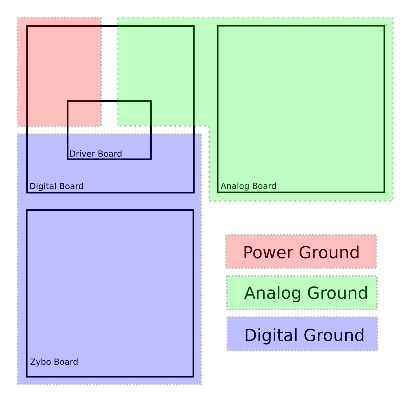
\includegraphics{graphics/ground_plane}
	\caption{Simplified view of the electronics with the ground planes marked.}
	\label{fig:groundplanes}
\end{figure}
\todo[inline]{Mikkel: I don't think all the TEN20-4823WIN ect. names should be here.}
As it is undesirable to have the potentially noisy GNDP present on the boards, it is constrained to one corner of the digital board.
Here it is used to supply the TEN20-4823WIN and the TVN5-4811WI isolated dc-dc converters that generate the $\pm15$\si{\volt} and 5\si{\volt} rails respectively.
The previously mentioned 3.3\si{\volt} rail is generated on the Zybo board.
The driver chip (The DRV8301 is discussed in more detail in section \ref{sec:driverboard}), is also supplied from the power rail, and as such GNDP is extended to a corner of the driver board.
Limiting the extent of GNDP is also the reasoning behind generating the $\pm15V$ rail on the digital board, even though it is used exclusively on the analog board.

\subsection{Analog Board}
The analog board houses, as the name implies, all of the analog signal processing.
Mainly the over-current protection, but also the torque pedal scaling is present on this board.

\subsubsection{Over-current Protection}
\label{sec:ocpcircuit}
In order to protect the system, it is necessary to create some form of over-current protection, OCP.
Two choices immediately present themselves:
\todo[inline]{Mikkel:Shut down the drivers= shut down gatesignals to FETS?.}
\begin{enumerate}
	\item The DRV8301 is equipped with current sensing circuitry that allows the chip to automatically shut down the drivers when an over-current event, OCE, occurs.
	\item External circuitry that, based on the measurements done by the current transducers, detects an OCE and turns off the drive signals by driving the EN\_GATE signal of the DRV8301 low. 
\end{enumerate}

Initially 1 seemed like a sensible choice, however, at the time it was not possible to deduce the functionality of the OCP in the DRV8301 based on the datasheet.
Therefore it was decided to use 2 since the function of the OCP will be well known and can be easily adjusted to meet any altered requirements, should the need arise.\\

In testing, the OCP function of the DRV8301 repeatedly shut down the drive circuitry and it was necessary to determine how to disable this feature.
During this research the functionality of the OCP was more well understood.
Due to difficulties with the debugging of the custom OCP circuitry presented below, it was decided to use the built-in OCP function of the DRV8301.
This is discussed in more detail in section \ref{sec:driverboard}.\\

Regardless of this change, it was decided to keep the description of the original OCP circuitry as this constitutes a significant portion of the work done on the project.
This description continues here:
Since only two phases are measured directly it is necessary to calculate the third.
This is done using a non-inverting summing amplifier.
See figure \ref{fig:sumamp}.
The output of this amplifier is given by:
\begin{equation}
	V_{out} = \left(1+\frac{R_4}{R_3}\right)\left(V_1\frac{R_2}{R_1+R_2}+V_2\frac{R_1}{R_2+R_1}\right)
\end{equation}

No amplification of the signals is wanted, thus the resistances are all set to $R=20k\Omega$. \todo{Thomas:Need correct values from Klaus/Martin}
With all three phase signals available it is possible to process them to detect any OCE's. 

\begin{figure}
	\centering
	\noindent\makebox[\textwidth]{\includegraphics[width=2\linewidth, trim=0cm 9cm 0cm 8cm]{graphics/sumamp}}
	\caption{The non-inverting summing amplifier used to calculate the current in the third phase.}
	\label{fig:sumamp}
\end{figure}

\begin{figure}
	\centering
	\includegraphics[width=\linewidth, trim=0cm 6cm 0cm 5cm]{graphics/ocp_phase}
	\caption{One phase of the over-current protection circuit.}
	\label{fig:ocpcircuit}
\end{figure}

The entire protection circuit for one phase can be seen in figure \ref{fig:ocpcircuit}.
Here the circuit has been split in accordance with the functionality of its four main parts: ADC isolation, full wave rectifier, thresholding circuit and an inverter.
Each part will be explained in appropriate detail in the following paragraphs.

\paragraph{ADC Isolation:}
The current measured in each phase is used in the control of the motor and as such it is important to maintain the integrity of the signal.
Therefore, after routing the signal to the ADC it is applied to the OCP circuit through a voltage follower.
Since the op amp has extremely high input resistance ($10^{12}$\si{\ohm} in the case of the LF353 used in this circuit) what happens on the output-side of the voltage follower has no meaningful impact on the input-side.

\paragraph{Full Wave Rectifier:}
The phase signals are sinusoids with an expected peak amplitude of $\pm0.5$\si{\volt}.
In order to only needing to detect a positive OCE the signal is rectified.
Due to the small magnitude of the signals it is necessary to use a precision full wave rectifier.
The rectifier used here can be divided into two subcircuits; a half-wave rectifier and a summing amplifier.
In order to show the functionality of the rectifier, three test points are marked on the circuit, $V_i$, $V_r$, and $V_o$.
$V_i$ is the input voltage, $V_r$ is the rectification stage and $V_o$ is the rectified signal.
Figure \ref{fig:rectifier} shows the voltages at these points.

\begin{figure}
	\centering
	\includegraphics[width=\linewidth]{graphics/rectifier}
	\caption{The condition of the signal at points $V_i$, $V_r$ and $V_o$ in the full wave rectifier.}
	\label{fig:rectifier}
\end{figure}
\todo[inline]{Thomas: It was my intention to explain the function of this full-wave rectifier but it somehow illudes me}
\paragraph{Thresholding:}
\label{sec:schmitt}
As explained in section \ref{sec:lemsensor}, the input signal to the OCP circuit is dimensioned such that the maximum current in either of the phases will result in a voltage of 0.5\si{\volt}.
Also mentioned in this section is the desire to leave some headroom in case of an OCE.
This is due to the response time of the system.
50\si{\milli\volt} is estimated to be sufficient.
An OCE is therefore defined as a time where the voltage exceeds 0.45\si{\volt}.
In order to avoid repeatedly switching the signal on and off, it was decided to use a Schmitt trigger.
Determining the component values is done using the following equations:

\begin{align}
	\frac{V_{cc}-V_h}{R_{7}}&=\frac{V_h}{R_8}+\frac{V_h-V_{ref}}{R_6} \label{eq:vhigh}\\
	\frac{V_{dd}-V_l}{R_{7}}&=\frac{V_l}{R_8}+\frac{V_l-V_{ref}}{R_6} \label{eq:vlow}
\end{align}

Where $V_{ref}=2.5$\si{\volt} as set by the LM4040\footnote{Precision 2.5\si{\volt} voltage reference}, the supply voltage $V_{cc}=15$\si{\volt}.
The desired hysteresis voltages $V_h$ and $V_l$ are $0.475$\si{\volt} and $0.25$\si{\volt} respectively.
This ensures that the enable signal will be pulled low when the current through any of the phases exceeds 285\si{\ampere}, and will not return until the current is below 150\si{\ampere}.
The LM4040 supplies a voltage in, effectively the same manner as a linear voltage supply.
It is therefore desirable to draw as little current from the component, that is, through $R_6$, as possible.
As per the datasheet it can operate from 60$\mu A\rightarrow15$\si{\milli\ampere}.
It was decided to set the maximum current through $R_6$, $\frac{V_{ref}-V_l}{R_6} = I_{R_6}=100$\si{\micro\ampere}.
This sets $R_6 = 22.5$\si{\kilo\ohm}.
$R_7$ and $R_8$ can now be isolated using \ref{eq:vhigh} and \ref{eq:vlow}:

\begin{align}
	R_7 &= \frac{(V_{cc}V_l-V_{dd}V_h)(V_l-V_{ref})}{I_{R_6}(V_h-V_l)V_{ref}}\label{eq:r7}\\
	R_8 &= \frac{(V_{cc}V_l-V_{dd}V_h)(V_l-V_{ref})}{I_{R_6}(V_{cc}(V_l-V_{ref})-V_{dd}(V_h-V_{ref})+(V_h-V_l)V_{ref})}\label{eq:r8}
\end{align}

Resulting in $R_7 = 150$\si{\kilo\ohm} and $R_8 = 2542.37$\si{\ohm}.
Since 2542.37\si{\ohm} is hardly a standard value, the nearest standard value is chosen such that $R_8=2550$\si{\ohm}.

\todo[inline]{Thomas: What do these rounded values result in, in terms of hysteresis}
\todo[inline]{Thomas: I think there is an error in the calculations vs the text - it seems the values result in 0.475 when we discussed 0.45 volt hysteresis.}

\paragraph{Inverter:}
Due to the NOR-stage described in section \ref{sec:nor}, it is necessary to invert the signal.
A simple comparator is used to achieve this effect.
The input voltage to this stage is either $V_{cc}$ or $GNDD$, the voltage on the non-inverting terminal is therefore not critical.
Setting $R_9=R_{10}=10$\si{\kilo\ohm} is sufficient.

The circuitry discussed above will ensure that in case of an OCE, a signal is sent to the digital board where it will be used to safely handle the event.
This is discussed in further detail in later sections. 

\subsubsection{Current Transducer - LF 205-S}
\label{sec:lemsensor}
While these current sensors are not strictly part of the analog board, the circuitry related to them is and therefore it was chosen to include their description here.
The LF 205-S utilises the Hall effect in order to measure the current flowing through a wire.
Figure \ref{fig:lf205function} depicts an equivalent circuit of the functionality of the transducer.
As can be seen, the LF 205-S functions like a transformer.
\todo[inline]{Mikkel: where is the figure?}
As per the datasheet this transformer has a 1:2000 turns ratio, therefore the secondary current, $I_S$ can be found as:
\begin{equation}
	\frac{I_S}{I_P}=\frac{N_P}{N_S} \quad \Rightarrow \quad I_S = \frac{I_P}{N_S}
\end{equation}
Essentially, the LF 205-S generates a current proportional to the current flowing through the device, the primary current; $I_P$.
By changing the value of the resistor $R_m$, the resulting voltage drop can be dictated.

In section \todo[inline]{Thomas: Section documenting the maximum current to be expected in each phase.} the maximum current to be expected in each phase is found to be 300$A$.
As will be described in section \ref{sec:emb}, the ADC on the Zynq chip can work on signals in the ranges 0\si{\volt}-1\si{\volt} or $\pm0.5$\si{\volt}.
Since the current is sinusoidal it can be negative.
Choosing the range $\pm0.5$\si{\volt} therefore simplifies the circuitry needed to read the value correctly.
Consequently $R_m$ needs to be set such that the maximum expected current results in the maximum allowed voltage.
However, it is desirable to leave some headroom in case of an OCE, 50\si{\milli\volt} should be sufficient.
Thus:
\begin{equation}
	R_m = \frac{0.45}{I_{Pmax}/N_S} = 3\Omega
\end{equation}
\todo[inline]{Mikkel: Should be updated with the real meaning of bipolar.}

\subsubsection{Torque Pedal Downscale}
The torque pedal is simply a variable resistor, $R_{tp}=7.5$\si{\kilo\ohm}. \todo[inline]{Thomas: Verify resistor value on final system}
As the pedal is actuated the resistance changes.
Figure \ref{fig:torquepedaldownscale} is a depiction of the circuit used to read the position of the torque pedal.

$R_1$ and $\mathrm{R_P}$ form a variable voltage divider of the 15\si{\volt} rail.
The analog input of the ADC in the FPGA, however, is limited to 0-1\si{\volt}.
Therefore it is necessary to downscale the voltage.
Intuitively this could be done using simply a voltage divider, but since the torque pedal functions as a voltage divider, the varying resistance distribution of the torque pedal would influence the voltage divider.
For this reason a voltage follower is used to isolate the two circuits.
In addition, a 5.1\si{\volt} zener diode is clamping the signal to ground in order to protect the ADC of the FPGA.
\todo{capacitor for noise}
\begin{figure}[!h]
	\centering
	\includegraphics[width=.75\linewidth]{graphics/torque_pedal_downscale}
	\caption{Circuit used to scale the voltage from the torque pedal from $0V\rightarrow5V$ to $0V\rightarrow1V$.}
	\label{fig:torquepedaldownscale}
\end{figure}

The resistance of the pedal is assumed to change linearly, which means the voltage division does not. 
Voltage at the point TP as a function of pedal is:

\begin{equation}
V_{TP}(R_P) = V_{CC} \frac{R_P}{R1 + R_P} \frac{R3}{R3 + R2}
\label{eq:pedal_voltage}
\end{equation}
\todo[inline]{Mikkel: Do we need so much whitespace in this figure?}
\todo[inline]{Mikkel: IS there a reason why numbers on resistors are not subscripted?.}
By isolating $\mathrm{R_P}$, it's possible to calculate what its resistance is. 
The resistance of $\mathrm{R_P}$ varies from $0$ to 7.5\si{\kilo\ohm}, as the pedal is pressed down. 
Hence, equation~\ref{eq:pedal_back_calc} will give a value proportional to the torque requested by the driver

\begin{equation}
R_P = \frac{V_{TP} R1 \cdot (R2 + R3)}{R3 \cdot (V_{CC} - T_{TP}) -  V_{TP} \cdot R2}
\label{eq:pedal_back_calc}
\end{equation}

Finally, due to the mechanical nature of the torque pedal, this signal is likely to be noisy.
C$_1$ is placed in order to filter this noise.

\begin{figure}[H]
	\begin{center}
		\includegraphics[width=10cm]{graphics/pedal_voltage.pdf}
		\label{fig:pedal_voltage}
		\caption{Voltage as a function of the pedal resistance.}
	\end{center}
\end{figure}

\subsection{Digital Board}
The digital board is used mostly as an interconnection board between the various electronic components in the system.
The logic levels of the different systems are managed here along with the enable signal for the DRV8301.
Additionally this board houses the in-rush relay.

\subsubsection{Drive Enable Signal}
This signal is produced by the torque pedal.
When the user actuates the pedal a switch is connected to ground. 
By reading the drive enable signal it is therefore possible to determine when the controller should be running, allowing a means for avoiding integral windup.
Since this signal is left floating when the pedal is not active, it can be routed directly to the Zybo, using the internal pull-up resistors.
\todo[inline]{Mikkel: It has nothing to do with windup, but reset .}
\todo[inline]{Thomas: Is the torque pedal active low or active high? Correct two places above to reflect the correct case}
\subsubsection{Driver Enable Circuit}
\label{sec:nor}
The DRV8301 is equipped with a pin called \texttt{EN\_GATE}.
If, while running, this pin is pulled low, the drive signals are immediately shut down.
\todo[inline]{Mikkel: Gate signals.}
This feature allows for fast and reliable shut down of the motor in case of any detected faults.
There are two different types of faults detected within the system, the aforementioned OCE and an over-temperature event, OTE.
In addition to these two a signal is routed from the Zybo which enables the digital part of the system to disable/enable the motor, should the need arise.
As there are three different signals that all need to connect to the same pin, they are all NOR'ed, as seen in figure \ref{fig:driveenablesignal}.

\begin{figure}[!h]
	\centering
	\includegraphics[width=\linewidth,trim=0cm 3cm 0cm 3cm]{graphics/driver_enable_signal}
	\caption{The NOR circuit that compares the three enable signals to determine whether the drive signals should be on.}
	\label{fig:driveenablesignal}
\end{figure}

The observant reader will notice that two 2-input NOR gates was used rather than one 3-input gate.
Reason for this is that the OTE protection was not implemented until after the components were ordered.
In order then to not need additional components it was decided to cascade the available component.
This cascading however does mean that it is necessary to invert the logic level of the signals OCE, and OTE.
OCE is inverted on the analog board while OTE is used to pull the signal to ground.
The two signals are both routed to the Zybo.
This is done such that it is possible to discern which event has triggered when the motor halts.

\subsubsection{Logic-Level Shifters}
Tracking the angular position of the rotor is done using an encoder mounted on the motor.
Upon receiving a clock signal the encoder will return the current position of the rotor.
The encoder module is an AM256 which, according to the datasheet, requires at least 3.5\si{\volt} for digital high input.
However, the Zybo uses 3.3\si{\volt} and the clock signal therefore needs to be shifted to the correct voltage level, 5\si{\volt}. 
A, B, Z and Data generated by the AM256 all need to be shifted down to 3.3\si{\volt} in order to protect the Zybo.
The circuit for these four signals can be seen in figure \ref{fig:lls}.
The buffer used for these signals is, as can be seen from the figure, the 74AHC125 which is a quad-buffer.
$V_{out}$ of this device is equal to $V_{cc}$, while $V_{in}$ can be any voltage from $0\rightarrow 5$\si{\volt}, by supplying it from the 3.3\si{\volt} rail it will therefore act as a logic level shifter.

\begin{figure}[!h]
	\centering
	\includegraphics[width=.5\linewidth,trim=0cm 1cm 0cm 1cm]{graphics/lls}
	\caption[Logic level shifter circuit.]{The 74AHC125 quad-buffer used to shift the logic level of the encoder from 5\si{\volt} down to the $3.3$\si{\volt} required by the Zybo. Due to an oversight, a buffer with an enable on each port was bought. This feature is unnecessary and they are always enabled.}
	\label{fig:lls}
\end{figure}

\subsubsection{In-rush Relay}
When first switching on the entire system, a considerable amount of current is required to charge the capacitors used on the inverter.
In order to protect the batteries and the system in general, it is necessary to limit the amount of current that is flowing to the capacitors until the voltage drop across them is reasonably small.
The main relay, when closed, acts as a short circuit between the batteries and the inverter.
Instead of closing this relay immediately, an additional relay is set in parallel.
This is the in-rush relay.
In series with the in-rush relay is placed a resistor which is dimensioned to limit the current sufficiently.
This circuit can be seen in figure \ref{fig:irrelay}.
\todo[inline]{Thomas: I guess we would like to actuyally have this calculation...}

\begin{figure}[!h]
	\centering
	\includegraphics[width=.5\linewidth,trim=0cm 4.5cm 0cm 0cm]{graphics/irrelay}
	\caption[In-rush relay.]{In-rush relay circuit. A small relay is driven from the Zybo in order to pre-charge the capacitors before switching the main relay.}
	\label{fig:irrelay}
\end{figure}

\subsection{Driver Board}
\label{sec:driverboard}
The third and final board created in this project is the driver board.
This board is made exclusively to house the DRV8301, the driver chip chosen for this project.
The reason for the seemingly superfluous board is that there is no equipment available capable of creating the small footprint of the chip.
Therefore this board is made by an external fabricator.\\
\todo[inline]{Mikkel: Can nobody make it? ;).}
The DRV8301 is a three-phase gate driver with a built-in buck converter.
Additionally it features both dead time control as well as over-current protection.
This chip is made specifically with driving PMAC motors in mind, making it an ideal candidate for this project.
Figure \ref{fig:drv8301pinout} shows the pinout of the DRV8301.
This will be used as a basis for a brief discussion of the features provided by the chip.

\begin{figure}[!h]
	\centering
	\includegraphics[width=.4\linewidth]{graphics/drv8301pinout}
	\caption{Overview of the pinout of the DRV8301.}
	\label{fig:drv8301pinout}
\end{figure}

\subsubsection{Buck Converter}
The DRV8301 is equipped with a buck converter capable of supplying up to 1.5\si{\ampere}.
It contains only the switching circuitry and the characteristics of the converter can be designed using external components.
For instance, the voltage can be adjusted using the VSENSE pin.
According to the datasheet \cite{DRV8301} the buck converter is isolated from the remaining circuitry.
These aspects makes it an ideal candidate for creating the 5\si{\ampere} rail needed to supply the Zybo board.
Initially this was the intention, however, this introduced significant complications in terms of the grounding layout and it was decided to use the TVN5-4811WI described previously.
This decision led to a simpler grounding plane as well as a simpler driver board, both desirable outcomes.

\subsubsection{Over-Current Protection}
As has already been discussed, the functionality of the over-current protection of the DRV8301 was initially decided against, mainly due to the apparent complexity of the feature.
It was believed that this feature relied on the use of shunt resistors on the source pin of the low-side of two of the half-bridges.
Since this feature was not to be used the (believed to be) associated pins SN1, SP1, SN2 and SP2 were pulled to ground.
This was believed to disable the effects of the OCP.
In testing the driver board the nOCTW pin was repeatedly pulled low, indicating that an OCE had occured.
One feature of the OCP is the ability to disable it using SPI.
In attempting this, much was learned about its functionality.\\

The OCP detects an OCE by measuring $V_{ds}$.
$V_{ds}$ for the high side of either channel is measured between pin SH\_x and PVDD1 while the low side $V_{ds}$ is measured between SL\_x and SH\_x.
$R_{ds(on)}$ is known from the MOSFETs the threshold $V_{ds}$ for any $I_{ds}$ can be determined:
\begin{equation}
	V_{ds} = R_{ds(on)}\cdot I_{ds}
\end{equation}
Since the maximum $I_{ds}=300$\si{\ampere} and $R_{ds(on)}=3.2$\si{\milli\ohm} for the IRFP4468PBF (the MOSFET chosen for the inverter, see section \ref{sec:mosfet}):
\begin{equation}
	V_{ds} = 0.96\si{\volt}
\end{equation}
Clearly, it is necessary to set the correct threshold of $V_{ds}$.
This parameter as well as several others can be set using SPI.

\subsubsection{SPI}
The DRV8301 is capable of performing SPI communication as a slave.
As mentioned above, this can be used to change various parameters concerning the functionality of the chip.
When sending a message to the driver, it will respond in the following communication cycle with the appropriate information.
Figure \ref{fig:spipacket} is a depiction the format of an SPI input data packet.
Any message sent to the driver must adhere to this format.
As can be seen, the first 11 bits are data, followed by 4 address bits and finally, a read/write bit.

\begin{figure}[!h]
	\centering
	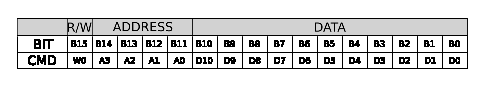
\includegraphics[width=\linewidth]{graphics/spipacket}
	\caption{SPI input data packet format of the DRV8301.}
	\label{fig:spipacket}
\end{figure}
\begin{figure}[!h]
	\centering
	\includegraphics[width=\linewidth]{graphics/spipacketresponse}
	\caption{SPI output data packet format of the DRV8301.}
	\label{fig:spipacketresponse}
\end{figure}

Figure \ref{fig:spipacketresponse} is a depiction of the format of an SPI output data packet.
Upon receiving a message on SDI a response is prepared in this format.
In a response packet, the R/W bit is used as a fault bit, indicating whether the received packet is valid.
\begin{figure}[!h]
	\begin{subfigure}[b]{\linewidth}
		\centering
		\includegraphics[width=\linewidth]{graphics/statreg1}
		\caption{Status register 1 of the DRV8301.}
		\label{fig:statreg1}
	\end{subfigure}
	\\
	\begin{subfigure}[b]{\linewidth}
		\centering
		\includegraphics[width=\linewidth]{graphics/statreg2}
		\caption{Status register 2 of the DRV8301.}
		\label{fig:statreg2}
	\end{subfigure}
	\caption{These registers contain the error bits of the system.}
	\label{fig:statreg}
\end{figure}
For a data packet to be considered valid, the DRV8301 requires the following:
\begin{itemize}
	\item SCLK must be low when $\overline{\text{SCS}}$ goes low.
	\item Packet must have 16 full clock cycles.
	\item SCLK must be low when  $\overline{\text{SCS}}$ goes high.
\end{itemize}

If the received packet is of type WRITE, the data in the response will contain the contents of status register 1, see figure \ref{fig:statreg1}.
Using a READ message the contents of any of the four registers can be read at any time.\\

All of the control of the functionality of the DRV8301 can be done through the control registers as seen in figure \ref{fig:contreg}.
Of interest to this project are OCP\_MODE and OC\_ADJ\_SET. 
OCP\_MODE allows the user to set the mode of operation of the OCP. 
One of four options can be chosen: current limit mode, OC latch shut down mode, report only mode and OC disabled mode.
During testing the driver was being run in OC disabled mode, however, during this time it was decided to attempt using the feature for detection of OCE's.
The OC\_ADJ\_SET allows setting the value of $V_{ds}$ appropriate for the type of MOSFET chosen.
As previously mentioned, this value is equal $V_{ds}=0.96$\si{\volt}.
Figure \ref{fig:vdstable} shows the different values that can be set as the threshold.
Since 0.96\si{\volt} is not available, the nearest value below is chosen.
Choosing a value above would result in an OC limit higher than the 300\si{\ampere} specified.	\todo[inline]{Thomas: Are we sure that it is 300 ampere in the calculations? why not 150 when the fets are parallelised?}
For this reason, the threshold is set to $V_{ds}=0.926$\si{\volt} by setting OC\_ADJ\_SET in control register 1 equal to 23.

\begin{figure}
	\centering
	\includegraphics[width=\linewidth]{graphics/vdstable}
	\caption{The threshold values for $V_{ds}$ and the associated code to be set in control register 1.}
\end{figure}

\begin{figure}[!h]
	\begin{subfigure}[b]{\linewidth}
		\centering
		\includegraphics[width=\linewidth]{graphics/contreg1}
		\caption{Control register 1 of the DRV8301.}
		\label{fig:contreg1}
	\end{subfigure}
	\\
	\begin{subfigure}[b]{\linewidth}
		\centering
		\includegraphics[width=\linewidth]{graphics/contreg2}
		\caption{Control register 2 of the DRV8301.}
		\label{fig:contreg2}
	\end{subfigure}
	\caption{These registers are used to control the functionality of the DRV8301.}
	\label{fig:contreg}
\end{figure}
